\section{Problema G - Error de la interpolación}\label{sec:interp_err}

Se define el error de una interpolación como
$$E(x) = \frac{ f^{n+1}(\xi) }{ (n+1)! } \prod_{i=0}^{n}(x - x_i) $$

donde $n$ es el grado del poliniomio interpolante, $f^{(n+1)}$ la derivada $n+1$ de la función y $\xi$ pertenece al intervalo que contiene todos los puntos utilizados. 

Represente gráficamente, en el intervalo adecuado y para las aproximaciones del apartado C) y D), las funciones de error dadas por la fórmula anterior usando aquellos valores
de $\xi$ que, dentro del intervalo considerado, la maximizan y la minimizan. Obtenga también las cotas de error que podemos extraer para esas aproximaciones.

\subsection{Resolución}

Primero tomaremos las primeras cuatro derivadas:

\begin{align}
	\partial_{\mu} f(\mu)
	&= - \frac{1}{\mu} C  \\
	\partial_{\mu}^{2} f(\mu)
	&= \frac{1}{\mu^2} C \\
	\partial_{\mu}^{3} f(\mu)
	&= \frac{-2}{\mu^3} C \\
	\partial_{\mu}^{4} f(\mu)
	&= \frac{6}{\mu^4} C	
\end{align}
\newpage

\subsubsection{Error cuadrático}

El error en la aproximación cuadrática es dado por la función:

$$ E_{cuad} = \frac{ \partial_{\mu}^3(\xi) }{3!} \prod_{i=0}^{2} (x - x_i) $$

Queremos encontrar pues, dos $\xi$ tal que $\partial_{\mu}^3(\xi)$ sea máxima o mínima en el intervalo $[0.78, 0.92]$.

\paragraph{Valores $\xi_{min}, \xi_{max}$}

Encontrar los valores $[\xi_{min}, \xi_{max}]$ no es tan complicado si observamos que se trata de $\partial_{\mu}^3(\xi) \approx -2\mu^{-3} $. Por ende los extremos del intervalos son también los extremos de $\partial_{\mu}^3(\xi)$ en ese intervalo.

\paragraph{Resultado}


A continuación se han visualizado la función de error para los dos valores de $[\xi_{min}, \xi_{max}]$. Como se puede ver, el error es de magnitud bastante inferior al rango de interés (miles de años).


\begin{figure}[H]
	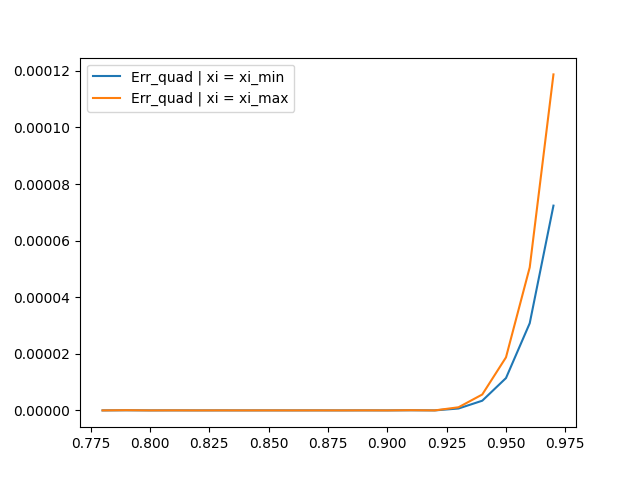
\includegraphics[width=\linewidth]{figures/figure6.png}
	\caption{Error en la aproximación cuadrática}
	\label{fig:err_cuad}
\end{figure}


\subsubsection{Error cúbico}

El error en la aproximación cúbica es dado por la función:

$$ E_{cub} = \frac{ \partial_{\mu}^4(\xi) }{4!} \prod_{i=0}^{3} (x - x_i) $$

Queremos encontrar pues, dos $\xi$ tal que $\partial_{\mu}^4(\xi)$ sea máxima o mínima en el intervalo $[0.78, 0.92]$.

Seguiremos una metodología parecida a la sección anterior.

\paragraph{Valores $\xi_{min}, \xi_{max}$}

Encontrar los valores $[\xi_{min}, \xi_{max}]$ no es tan complicado si observamos que se trata de $\partial_{\mu}^4(\xi) \approx 6\mu^{-4} $. Por ende los extremos del intervalos son también los extremos de $\partial_{\mu}^3(\xi)$ en ese intervalo.

\paragraph{Resultado}

A continuación se han visualizado la función de error para los dos valores de $[\xi_{min}, \xi_{max}]$. Como se puede ver, el error es de magnitud bastante inferior al rango de interés (miles de años).

\begin{figure}[H]
	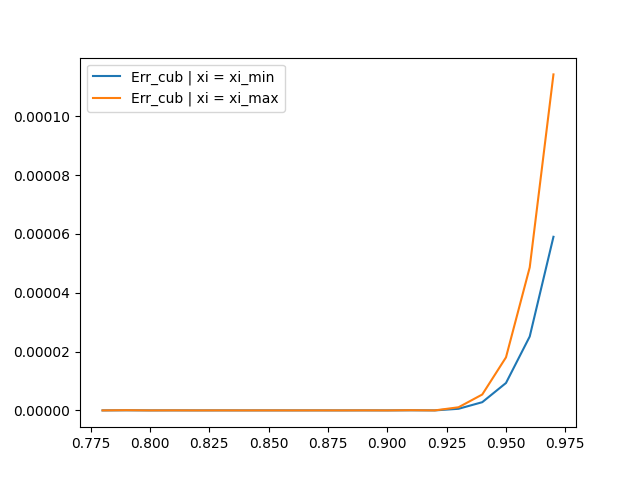
\includegraphics[width=\linewidth]{figures/figure7.png}
	\caption{Error en la aproximación cúbica}
	\label{fig:err_cub}
\end{figure}


\newpage

\subsubsection{Código}

El código utilizado para este ejercicio es:

\lstinputlisting[language=Python]{../../code/pecs/pec3/ex7.py}




\newpage

\subsubsection{Discusión}


Como se puede ver, los polinomios de orden $n = 2$ y $n = 3$ dan resultados similares. 

Los errores calculados son:

\begin{table}[htbp]
	\centering
	\csvreader[
	tabular=|c|c|c|,
	table head=\hline \textbf{Error} & \textbf{Value} \\\hline,
	late after last line=\\\hline,
	]{data/errors06.csv}{}{\csvlinetotablerow}
\end{table}

\paragraph{Error relativo}
Los valores aproximados estan en el orden de $f(x) \approx 10^{3}, ~ \forall x \in [0.78, 0.92]$. Considerando que el error de aproximación se ha visto que está por el orden de $E(x) \approx 10^{-9}, ~ \forall x \in [0.78, 0.92]$.

\subparagraph{Magnitud}

La magnitud del error relativo es aproximadamente:

\begin{align*}
	\frac { E(x) } { f(x) } 
	&\approx \frac{10^{-9}}{10^3}
	= 10^{-12}
\end{align*}

Lo que nos inspira bastante confianza en la edad obtenida por la interpolación.

\paragraph{Selección de datos}
Si nos encargamos de que los polinomios se construyan con los datos mas cercanos de los puntos de interés, podremos tener una aproximación relativamente buena.


Una buena manera de entender esto es ver que la interpolación de Lagrange usa la información contenida en un intervalo, que contrasta con otras formas de aproximar una función como la aproximación por polinomios de Taylor, donde la información se encuentra en el punto y las derivadas de $x$.

